% =============================================================================
% CONFERENCE PAPER (single file, <= 6 pages incl. references)
%
% Overleaf setup:
%   1. Paste this file as main.tex.
%   2. Create a folder "figures" and upload from NEW WAY/docs/figures/:
%        sece_phase3_architecture.png
%        benchmark_3h_heldout.png
%        case_study_laila_trajectories.png
%
% References are copied VERBATIM from the reviewed submission source
%   Paper Writing/After_Rejection Part/REVISION/Paper.tex
% Methodology citations (cawley2010, efron1979, wilcoxon1945, etc.) added as
% verified \bibitem entries beyond the ICCACCESS block; see bibliography end.
% Overleaf: Recompile twice so \cite{} and Fig.~\ref{} PDF links resolve.
% =============================================================================
\documentclass[conference]{IEEEtran}

\usepackage[T1]{fontenc}
\usepackage[utf8]{inputenc}
\usepackage{graphicx}
\graphicspath{{figures/}}
\usepackage{booktabs}
\usepackage{multirow}
\usepackage{amsmath}
\usepackage{cite}
\usepackage{url}
% Clickable in-text citations and figure/table links (compile twice in Overleaf).
\usepackage[hidelinks,breaklinks=true]{hyperref}
\hypersetup{pdfpagelabels=false,bookmarksnumbered=true}
\usepackage{flushend}

\newcommand{\sece}{SECE}
\newcommand{\bob}{Bay of Bengal}
\newcommand{\era}{ERA5}
\newcommand{\ibtracs}{IBTrACS}

% This paper is float-dense (2 tables, 4 figures in 6 pages). Default LaTeX
% allows at most 3 floats per page, which pushes figures far past the text that
% discusses them; these limits let each float settle at the top of a nearby
% column. The wide architecture diagram is a figure* so it spans both columns.
\setcounter{topnumber}{3}
\setcounter{bottomnumber}{2}
\setcounter{totalnumber}{5}
\renewcommand{\topfraction}{0.92}
\renewcommand{\bottomfraction}{0.8}
\renewcommand{\textfraction}{0.07}
\renewcommand{\floatpagefraction}{0.72}

\begin{document}

\title{ERA5-Augmented Ensemble Learning for Multi-Horizon Tropical Cyclone
Track Prediction over the Bay of Bengal: A Leakage-Aware Benchmark}

\author{\IEEEauthorblockN{Anonymous Submission}}

\maketitle

\begin{abstract}
Track guidance for \bob{} tropical cyclones underpins evacuation timing along one
of the world's most exposed coastlines, yet full numerical weather prediction is
costly for national agencies in the region. We benchmark eight tree-based track
predictors at 3, 12, 24, and 48\,h lead times on North Indian Ocean \ibtracs{}
storms with genesis in 1940--2024, augmenting 49 kinematic features with 14
\era{} reanalysis fields collocated at the storm centre. The proposed
Subset-Expert Context-Aware Ensemble (\sece{} v2 Phase~3) routes horizon-specific
subset experts, including a dedicated atmospheric ``environ'' expert, through
validation-only non-negative least squares fusion. We also report and correct a
test-set leakage mode of our own making: architectural phases had been advanced
while inspecting test-set rank tables, so we froze the design on nine development
seeds and evaluated nine disjoint held-out seeds exactly once. On the held-out
confirm (442 distinct test storms pooled), \sece{} attains median great-circle
errors of 4.895, 35.538, 101.186, and 246.331\,km. Paired Wilcoxon signed-rank
tests with Bonferroni correction show \sece{} is significantly better than all
seven baselines at 3 and 12\,h, statistically indistinguishable from the leading
stacks at 24 and 48\,h, and never significantly worse than any baseline at any
horizon. Ablations attribute long-lead gains to \era{}, while 5$^\circ$/3$^\circ$
spatial patch statistics were tested and rejected. CNN-GRU and BLSTM are omitted
from the locked confirm table after trailing tree-based systems in exploratory
development under the same uniform-hyperparameter protocol~\cite{grinsztajn2022tree}.
\end{abstract}

\begin{IEEEkeywords}
Tropical cyclone track prediction, ERA5 reanalysis, ensemble learning, Bay of
Bengal, IBTrACS, evaluation protocol, data leakage.
\end{IEEEkeywords}

\begin{figure}[!t]
\centering
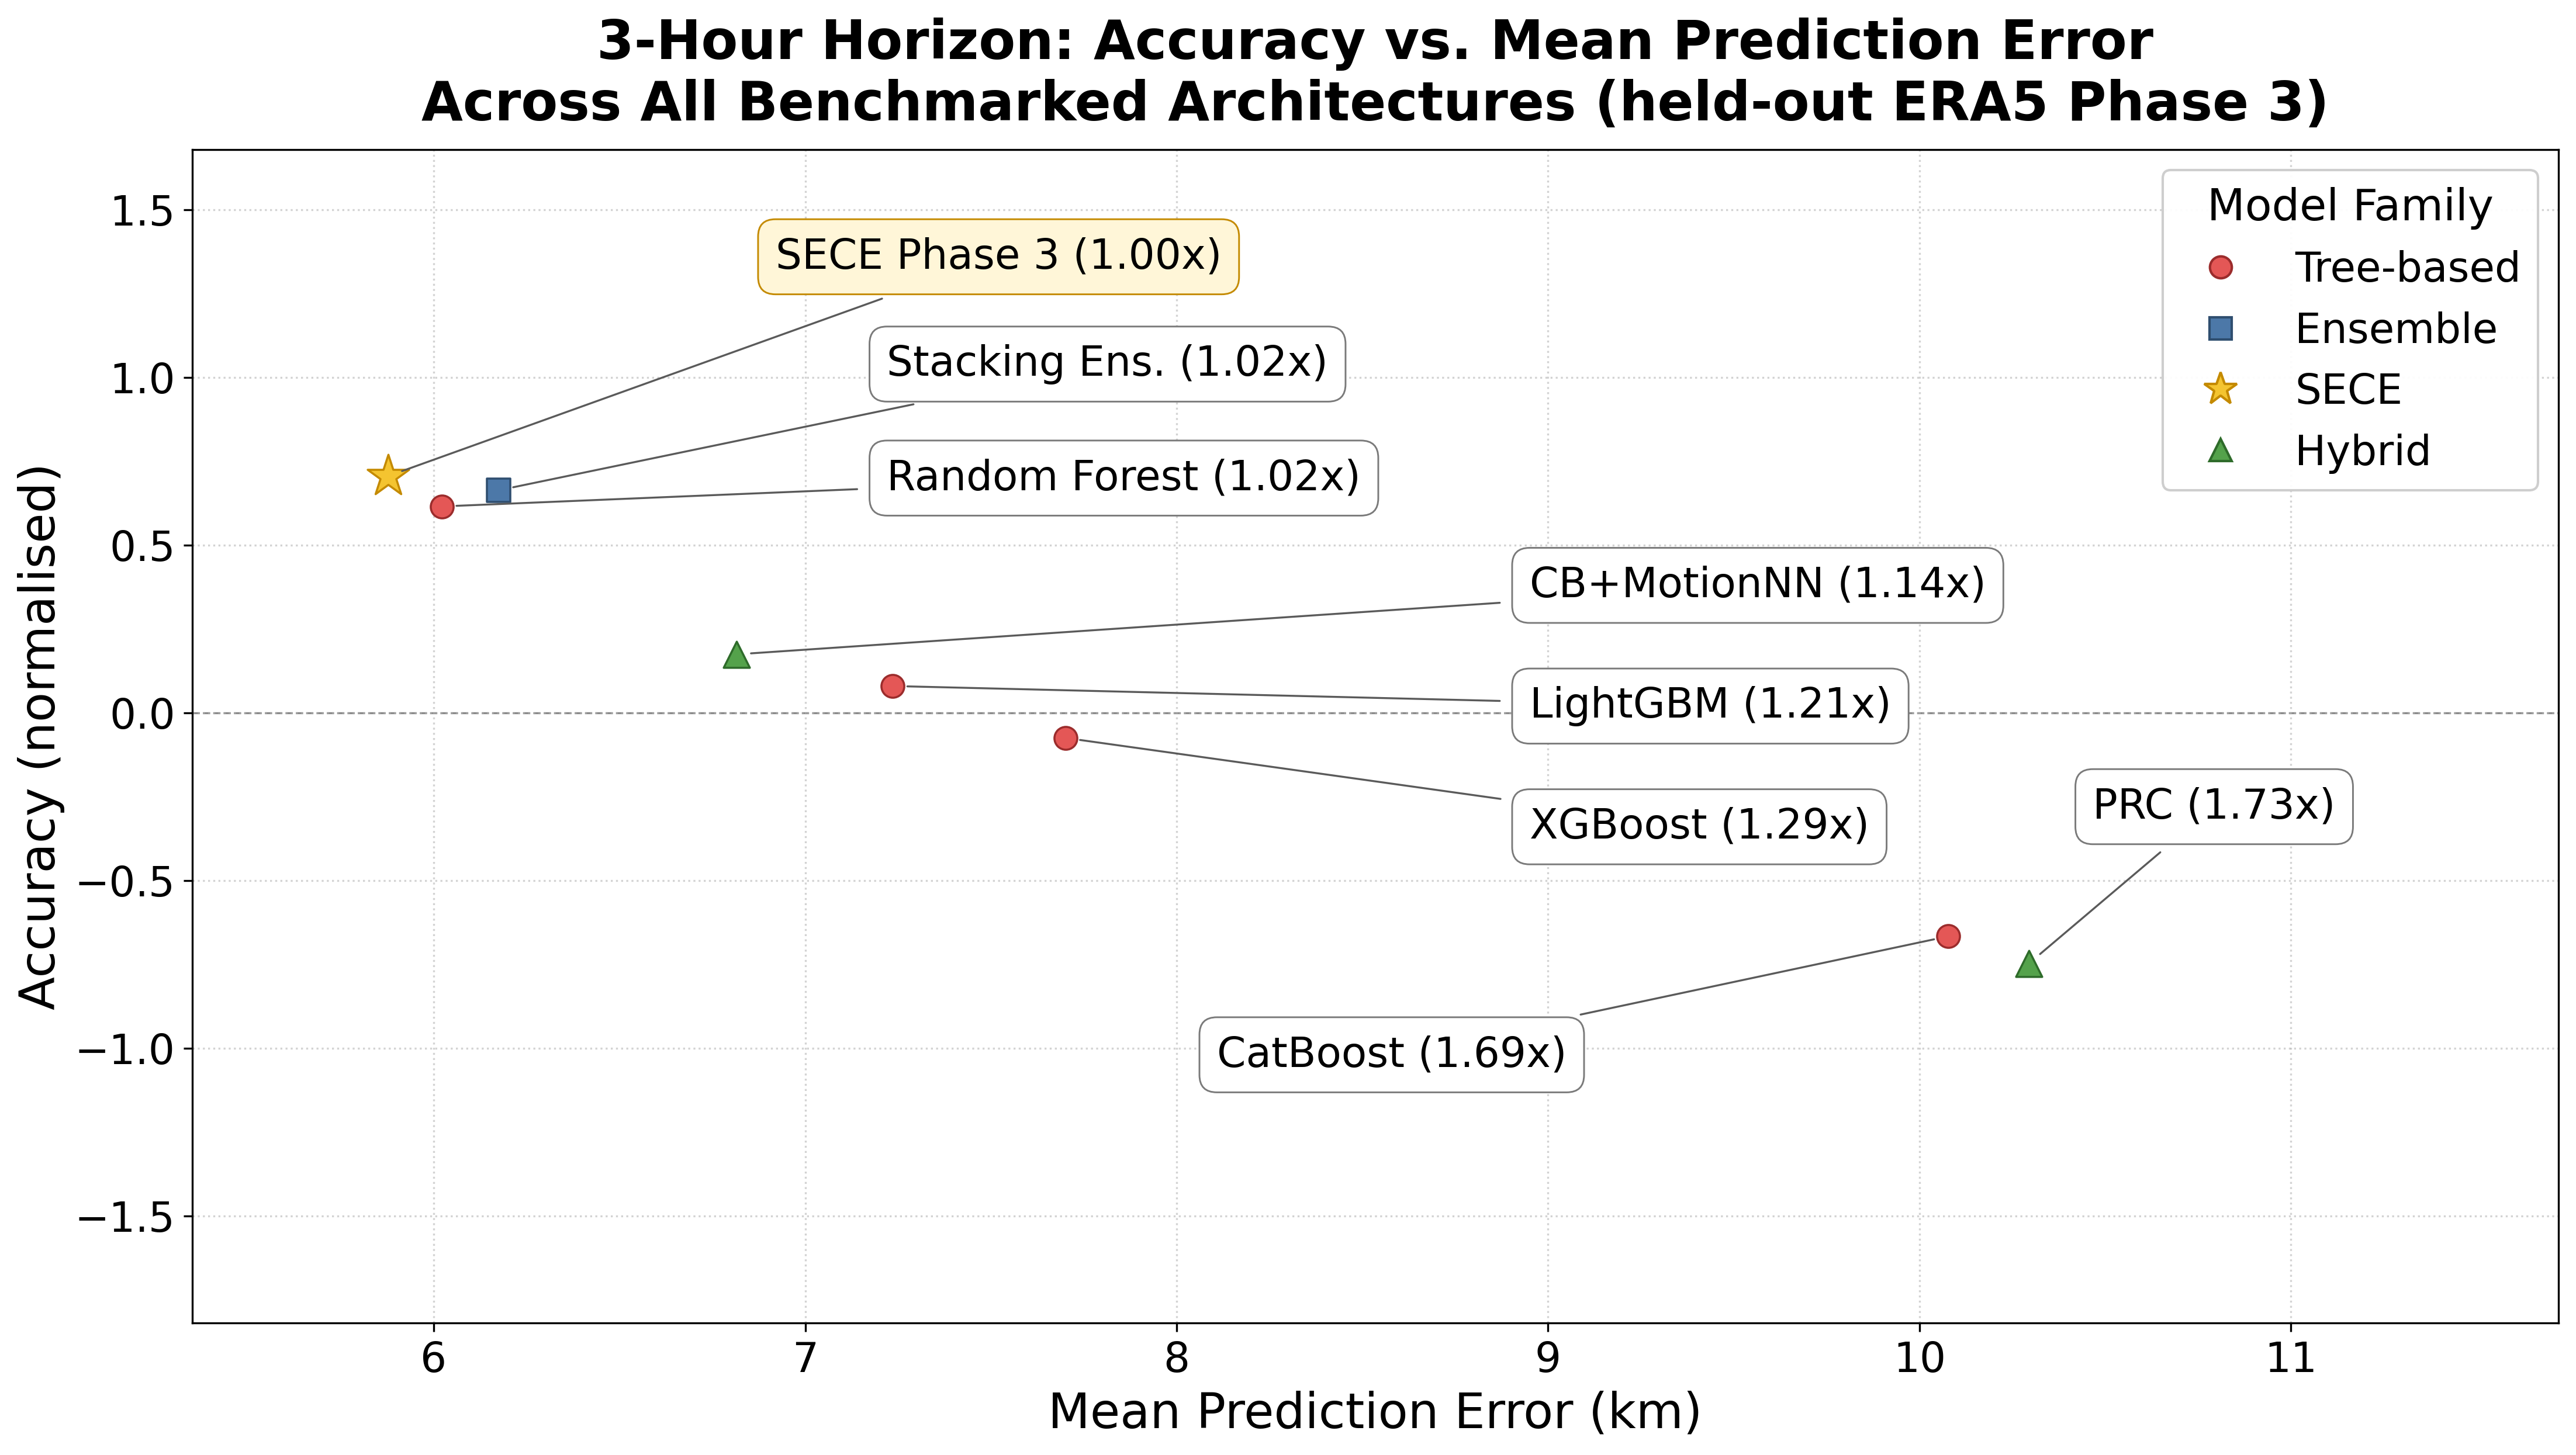
\includegraphics[width=\linewidth]{Figures/benchmark_3h_heldout.png}
\caption{Held-out 3\,h benchmark (pooled nine seeds). Horizontal axis: mean
great-circle error (km); vertical axis: normalised accuracy from \emph{median}
error vs.\ the tree family. Table~\ref{tab:held} reports pooled medians with 95\%
bootstrap CIs.}
\label{fig:bench}
\end{figure}

% =============================================================================
\section{Introduction}
% =============================================================================
\IEEEPARstart{T}{he} \bob{} concentrates a disproportionate share of global
tropical cyclone fatalities into a shallow, funnel-shaped basin bordered by
densely populated deltaic coastline. Cyclone Sidr in 2007 and the storm-surge
events that followed it drove sustained investment in early warning, for which
track uncertainty is the quantity that sets evacuation lead
time~\cite{worldbank2007sidr,paul2013post,dube2009storm}. Operational guidance
rests on dynamical models and consensus aids~\cite{goerss2000tropical,goerss2004tropical},
but the computational and assimilation infrastructure they require is not
uniformly available to national meteorological agencies in the region.

Data-driven track models offer a complementary path. Best-track archives supply
decades of labelled trajectories~\cite{knapp2010ibtracs,gahtan2024ibtracs}, and
global reanalysis supplies a physically consistent estimate of the atmospheric
state at each storm position~\cite{hersbach2023era5}, so a learned model can
consume environmental context without running a forecast
cycle~\cite{giffard2020tropical,kumar2024machine}. Reported approaches span
climatological-persistence analogues~\cite{neumann1972alternative,aberson1998five},
recurrent and convolutional sequence
models~\cite{lian2020novel,alemany2019predicting,rahman2025tropical}, and
transformer variants~\cite{qu2025accurate}. On engineered tabular data at the
sample sizes available for a single basin, however, tree ensembles remain hard to
displace~\cite{grinsztajn2022tree,ganaie2022ensemble}.

Three gaps motivate this work. First, basin-specific benchmarks for the North
Indian Ocean typically compare few architectures, so relative claims are
fragile~\cite{kar2021tropical,hossain2021track}. Second, evaluation is often
confined to a single lead time, leaving horizon-dependent behaviour
undocumented~\cite{kumar2024machine}. Third, the incremental value of reanalysis
over pure kinematics is rarely isolated by controlled ablation. A fourth gap is
methodological rather than architectural: when ensemble design is refined while
the designer inspects test-set rankings, the reported held-out estimate is
optimistic even though no model ever saw a test
label~\cite{cawley2010}.

This paper contributes an eight-system benchmark across four horizons under
storm-wise splits, bootstrap confidence intervals, and paired significance
testing; the \sece{} Phase~3 architecture with a dedicated \era{} environ expert
and validation-only routing; a documented correction of the leakage mode above,
including the fact that our pre-correction results did not replicate; and a
controlled ablation reporting the rejection of spatial patch features as a
negative result.

Deep sequence baselines (CNN-GRU, BLSTM) were scoped out after exploratory
development under the same fixed budget as the trees (300 estimators/epochs,
lr~0.01): both trailed tree and hybrid leaders at 3--24\,h~\cite{grinsztajn2022tree},
so the locked confirm lists eight tree systems only (Table~\ref{tab:held}).

% =============================================================================
\section{Data and Features}
% =============================================================================
\subsection{Archive, quality control, and splits}
We use \ibtracs{} v4 North Indian Ocean best
tracks~\cite{knapp2010ibtracs,gahtan2024ibtracs}. After quality control on
3-hourly rows, which enforces consistent timesteps and valid displacement
targets, the modelling table contains 852 storms and 27{,}728 forecast origins.
Multi-horizon supervision at 12, 24, and 48\,h requires a sufficient forward
track within each storm; 583 storms satisfy this and yield 15{,}605 multi-horizon
origins. Because storm assignment is fixed once at the multi-horizon level, all
four horizons draw from the same storm pool.

Partitioning is by storm identifier rather than by observation, so
autocorrelation within a trajectory cannot cross partitions. Each seed draws a
70:15:15 storm-wise split, which yields 408 training, 87 validation, and 88 test
storms per seed; sample counts vary with the length distribution of the storms
drawn, for example 11{,}066 training and 2{,}370 test multi-horizon samples on
seed~0.

\subsection{ERA5 collocation}
\era{} fields~\cite{hersbach2023era5} are extracted over
30$^\circ$N--5$^\circ$N, 70$^\circ$E--102$^\circ$E at 3-hourly resolution for
every day on which a tracked storm was active, and joined to each track row. The
14 point features are zonal and meridional wind at 850, 500, and 200\,hPa, mean
sea level pressure, sea surface temperature, a derived deep-layer steering wind,
and vertical shear expressed as 200\,hPa minus 850\,hPa components together with
its magnitude. Because \era{} sea surface temperature is undefined over land,
near-coast rows are filled from the nearest valid ocean cell and flagged; the
flag is retained as a feature so the model can condition on the substitution.

The 49 kinematic and derived predictors cover lagged positions, translation speed
and bearing with sinusoidal encoding, acceleration, bearing curvature, seasonal
encoding, a latitude-and-bearing recurvature proxy, distance to land, and
landfall state, following established practice for this
basin~\cite{krishnamurti2010ann,lian2020novel}.

The subset-expert design assumes these features carve the data into physically
meaningful regimes, so we check that before modelling. Fig.~\ref{fig:tsne}
projects the 63-dimensional space with t-SNE~\cite{maaten2008tsne}, coloured
independently by storm nature, translation speed, latitude band, and displacement
magnitude. Coherent structure under all four colourings, not just one, indicates
the feature space separates distinct kinematic and environmental regimes.

\begin{figure}[!t]
\centering
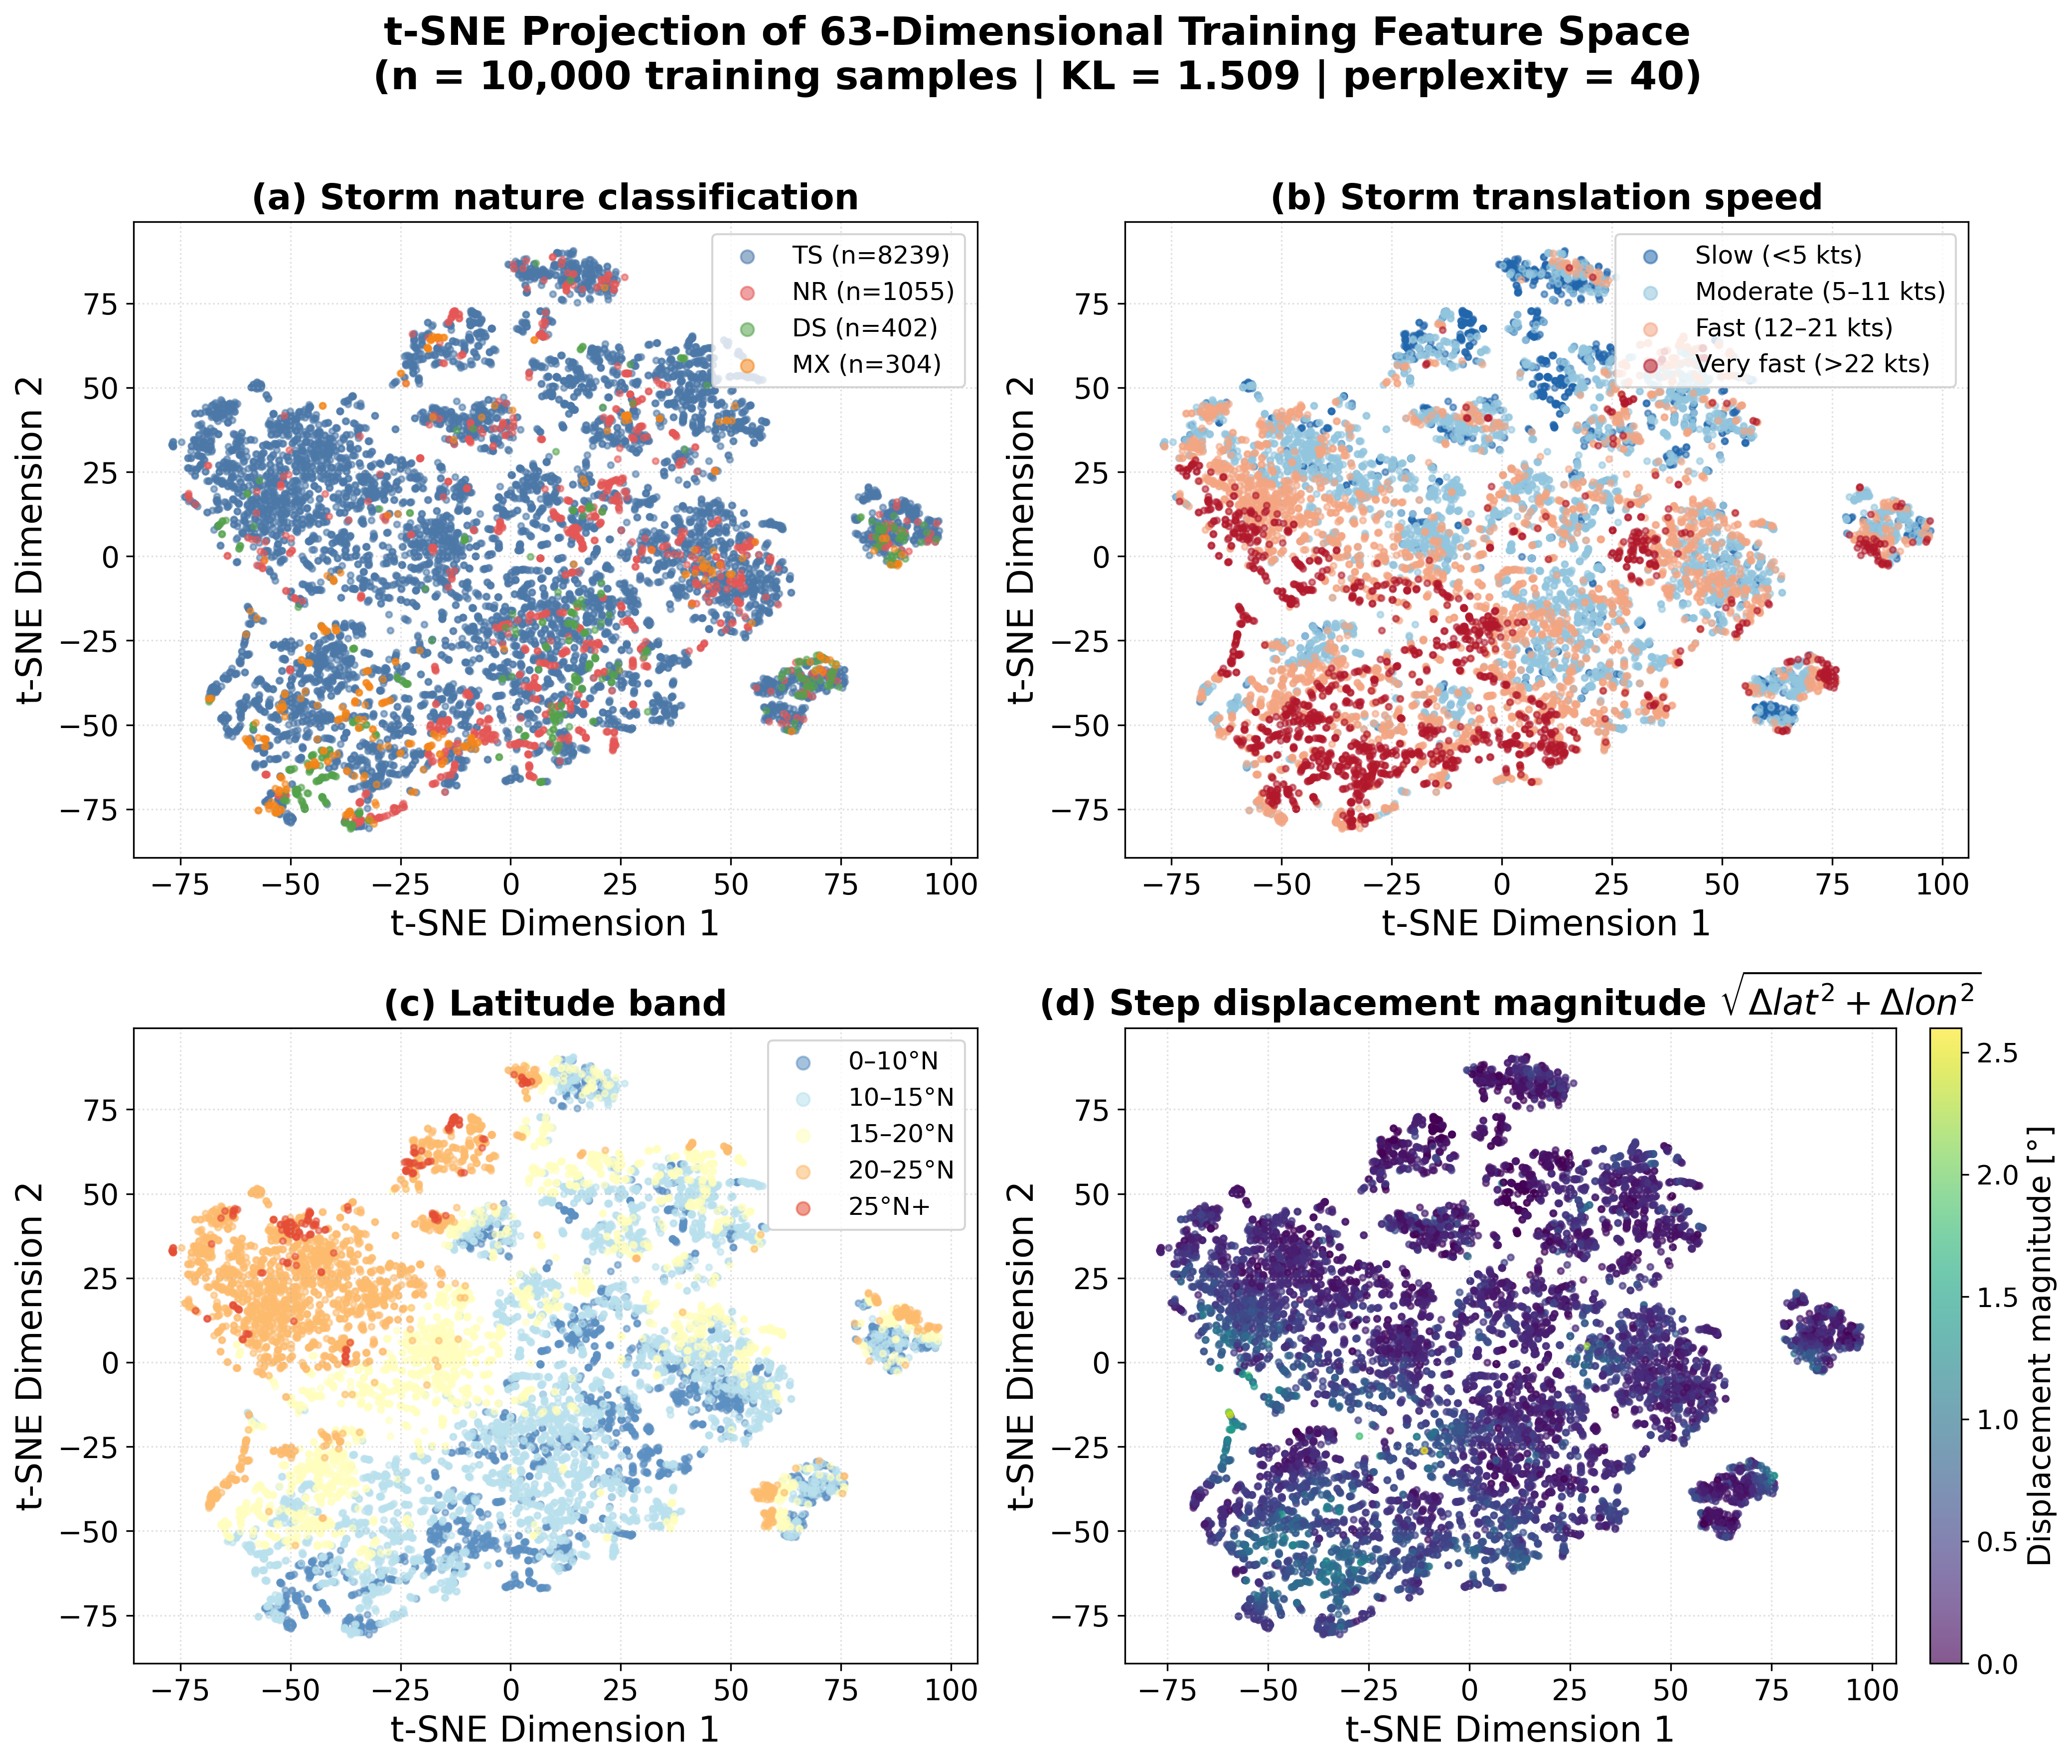
\includegraphics[width=\linewidth]{Figures/tsne_era5_63d.png}
\caption{t-SNE projection~\cite{maaten2008tsne} of the 63-dimensional feature
space ($n=10{,}000$), coloured by independent meteorological attributes.
Coherent separation indicates the engineered features encode physically distinct
regimes, which is the premise underlying the subset-expert design.}
\label{fig:tsne}
\end{figure}

\subsection{Genesis window}
We compared genesis windows of 1940--2024, 1979--2024, and 1990--2024. Because
observational quality improves sharply once satellite coverage begins, a naive
comparison confounds training-set size with test-set composition, so we repeated
the comparison with all three models evaluated on one common modern holdout. The
widest window won at every horizon on that fixed test, by 0.18\,km at 3\,h but by
7.9\,km at 24\,h and 17.7\,km at 48\,h relative to the modern-only model. We read
this as position records remaining usable in earlier decades even where intensity
observations are sparse, which suffices because the target here is track geometry
rather than intensity, and we lock 1940--2024 accordingly.

% =============================================================================
\section{Validation Protocol}
% =============================================================================
Early development advanced \sece{} through successive architectural phases on a
single fixed split, and the decision to advance from one phase to the next was
taken by inspecting per-horizon test-set rank tables and adding fusion paths that
closed the visible gaps. No test observation entered any fitting step, but the
architecture was selected using test feedback, which is sufficient to invalidate
the resulting held-out estimate~\cite{cawley2010}. The
concrete symptom was that a design which appeared to win at every horizon on the
original split did not reproduce that sweep on fresh splits.

We therefore separate two disjoint seed tiers. Nine development seeds
$\{3,4,5,6,8,9,10,11,14\}$ carry every architectural and fusion-path decision.
Nine held-out seeds $\{0,1,2,7,13,99,123,2024,2026\}$ were generated and
evaluated exactly once, after the architecture was frozen. Convergence is
verified by agreement between the tiers rather than by further tuning: at 48\,h
the development and held-out means differ by 0.05\,km (246.94 against
246.99\,km).

The primary metric is median great-circle error in kilometres, computed per test
storm and aggregated~\cite{sinnott1984}. The held-out confirm
adds 95\% confidence intervals from 10{,}000 storm-level bootstrap
resamples~\cite{efron1979} and paired Wilcoxon signed-rank
tests on matched per-storm medians~\cite{wilcoxon1945}, with
Bonferroni correction across the seven simultaneous
comparisons~\cite{bonferroni1936} giving a threshold of
$\alpha = 0.05/7 \approx 0.0071$.

% =============================================================================
\section{Method}
% =============================================================================
\subsection{Baselines}
Seven comparators span the tree and hybrid families: a Ridge-penalised stacking
ensemble over Random Forest, XGBoost, and LightGBM base learners; a Persistence
Residual Cascade (PRC) that corrects a persistence extrapolation with a LightGBM
residual fitted in kilometre space; Random Forest~\cite{breiman2001rf};
LightGBM~\cite{ke2017lightgbm}; XGBoost~\cite{chen2016xgboost};
CatBoost~\cite{prokhorenkova2018catboost}; and CB+MotionNN, a CatBoost predictor
corrected by a 64-32-16 multilayer perceptron acting on kinematic residuals. All
tree learners share 300 estimators, maximum depth 6, and learning rate 0.01, so
that differences reflect architecture rather than tuning
budget~\cite{grinsztajn2022tree}.

\begin{figure*}[!t]
\centering
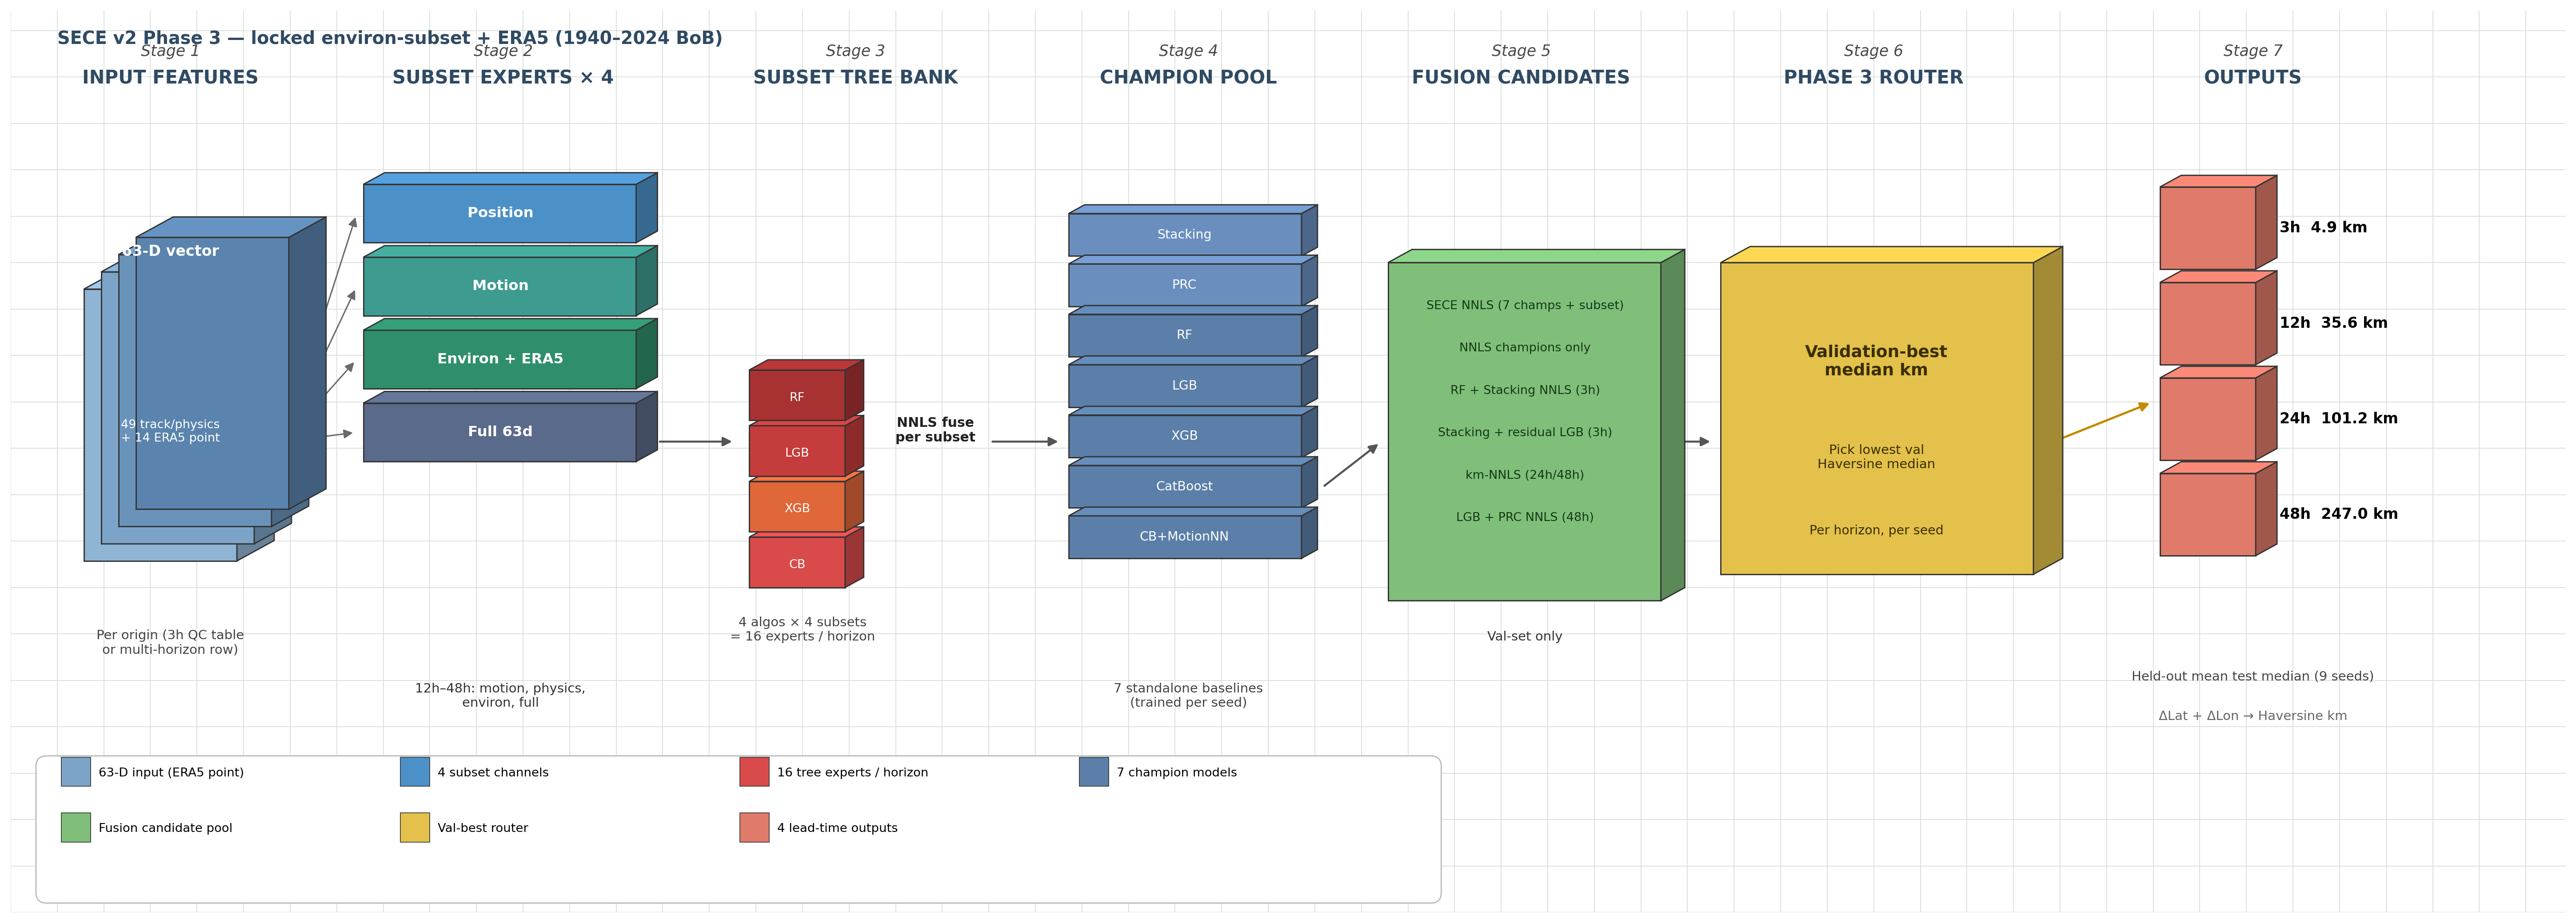
\includegraphics[width=0.98\textwidth]{Figures/sece_phase3_architecture.png}
\caption{Locked \sece{} Phase~3 pipeline. Sixty-three inputs, 49 kinematic and 14
\era{} point features, feed four horizon-specific subset experts, each modelled by
four tree algorithms and fused by non-negative least squares; a validation-only
router selects the final fusion candidate per seed.}
\label{fig:arch}
\end{figure*}

\subsection{SECE Phase~3}
For each horizon, \sece{} builds four physics-informed feature subsets, shown in
Fig.~\ref{fig:arch}. At 3\,h these are position, motion, environ, and the full
set; at 12, 24, and 48\,h they are motion, physics, environ, and full. Each
subset is modelled by all four tree algorithms, giving 16 subset-level models per
horizon, which are fused by non-negative least squares into one subset-consensus
signal. That signal joins the seven baseline predictions in a second-stage fusion
pool, from which horizon-specific candidates are formed: degree-space fusion over
the full pool, a persistence-anchored kilometre-space variant, and at 3\,h an
additional stacking-plus-residual path. A hard router then selects, per seed, the
candidate with the lowest \emph{validation} median error, and that frozen choice
produces the reported test predictions.

The environ expert is the locked architectural addition. Rather than dispersing
the 14 \era{} features into existing subsets, we allocate them, together with the
native environmental fields, to a dedicated subset with its own four-algorithm
pool. This gives atmospheric information explicit representation in the ensemble
and was selected over the alternatives in Section~\ref{sec:abl}.

% =============================================================================
\section{Results}
% =============================================================================
\subsection{Development ablation}
\label{sec:abl}
Table~\ref{tab:abl} reports, per configuration, the number of development seeds
on which \sece{} ranked first among all eight systems, and its mean median error.
Adding point \era{} features reduces the 48\,h mean from 250.26 to 246.80\,km,
with 8 of 9 seeds improving, which establishes that atmospheric information
carries exploitable signal at long lead. Routing those features through a
dedicated environ expert then improves 24\,h specifically, from 99.86 to
99.43\,km, which is the horizon at which the plain point-\era{} configuration was
weakest. The same table records an honest cost: at 3\,h the track-only
configuration retains the lowest mean, 4.84 against 4.93\,km, so \era{} does not
help uniformly across horizons.

Spatial patch statistics at 5$^\circ$ and 3$^\circ$ raise short-range rank-1
frequency but leave 24 and 48\,h means within roughly 0.4\,km of the environ
configuration, inside the seed-to-seed noise. We therefore did not adopt them,
and report the rejection rather than omitting it.

\begin{table}[!t]
\caption{Development ablation over nine development seeds. Each cell gives
\sece{} rank-1 count out of nine, then mean median error in km. The locked row is
in bold; the final row is the independent held-out confirm for reference.}
\label{tab:abl}
\centering
\footnotesize
\setlength{\tabcolsep}{3.5pt}
\begin{tabular}{@{}lcccc@{}}
\toprule
Configuration & 3\,h & 12\,h & 24\,h & 48\,h \\
\midrule
Track-only (no \era{})      & 5/9, 4.84 & 3/9, 35.48 & 3/9, 100.48 & 0/9, 250.26 \\
$+$ point \era{}            & 5/9, 4.93 & 7/9, 35.59 & 2/9, \phantom{0}99.86 & 1/9, 246.80 \\
\textbf{$+$ environ expert} & \textbf{5/9, 4.93} & \textbf{6/9, 35.56} & \textbf{3/9, \phantom{0}99.43} & \textbf{2/9, 246.94} \\
$+$ spatial 5$^\circ$       & 7/9, 4.93 & 7/9, 35.56 & 1/9, \phantom{0}99.74 & 1/9, 246.55 \\
$+$ spatial 3$^\circ$       & 7/9, 4.93 & 7/9, 35.66 & 2/9, \phantom{0}99.42 & 3/9, 247.00 \\
\midrule
Held-out confirm (locked)   & 6/9, 4.90 & 6/9, 35.63 & 2/9, 101.21 & 1/9, 246.99 \\
\bottomrule
\end{tabular}
\end{table}

\subsection{Held-out confirm}
\begin{table*}[!t]
\caption{Held-out test performance ranked at each horizon: model and median
great-circle error (km) with 95\% bootstrap confidence interval. Nine held-out
seeds pooled (442 distinct storm identifiers; 34{,}114 test samples at 3\,h and
21{,}442 at 12--48\,h). Eight tree/hybrid systems only; CNN-GRU and BLSTM omitted
(see Section~I).}
\label{tab:held}
\centering
\scriptsize
\resizebox{\textwidth}{!}{%
\begin{tabular}{@{}c lcc lcc lcc lcc@{}}
\toprule
\multirow{2}{*}{\textbf{Rank}} &
\multicolumn{3}{c}{\textbf{3\,h Horizon}} &
\multicolumn{3}{c}{\textbf{12\,h Horizon}} &
\multicolumn{3}{c}{\textbf{24\,h Horizon}} &
\multicolumn{3}{c}{\textbf{48\,h Horizon}} \\
\cmidrule(lr){2-4}\cmidrule(lr){5-7}\cmidrule(lr){8-10}\cmidrule(lr){11-13}
& \textbf{Model} & \textbf{Med.} & \textbf{95\% CI} &
\textbf{Model} & \textbf{Med.} & \textbf{95\% CI} &
\textbf{Model} & \textbf{Med.} & \textbf{95\% CI} &
\textbf{Model} & \textbf{Med.} & \textbf{95\% CI} \\
\midrule
1 & \textbf{\sece{}} & \textbf{4.895} & 4.71--5.08 &
\textbf{\sece{}} & \textbf{35.538} & 34.2--36.9 &
Stacking & 100.771 & 96.9--104.7 &
XGBoost & 242.702 & 232.6--255.4 \\
2 & RF & 4.927 & 4.73--5.13 &
Stacking & 36.146 & 34.7--37.7 &
XGBoost & 101.029 & 96.9--105.3 &
PRC & 243.229 & 231.7--255.2 \\
3 & Stacking & 4.945 & 4.76--5.12 &
RF & 36.901 & 35.5--38.3 &
\textbf{\sece{}} & \textbf{101.186} & 97.3--104.8 &
LGB & 245.975 & 234.9--257.2 \\
4 & CB$+$MoNN & 5.813 & 5.70--5.93 &
LGB & 36.928 & 35.5--38.3 &
LGB & 101.632 & 97.8--105.6 &
Stacking & 245.977 & 235.9--257.2 \\
5 & LGB & 6.026 & 5.89--6.17 &
XGB & 36.947 & 35.5--38.4 &
PRC & 101.941 & 98.1--105.8 &
\textbf{\sece{}} & \textbf{246.331} & 235.5--257.6 \\
6 & XGB & 6.411 & 6.24--6.58 &
PRC & 37.177 & 35.7--38.5 &
RF & 103.511 & 99.7--107.4 &
CB$+$MoNN & 249.678 & 239.0--261.2 \\
7 & CatBoost & 8.479 & 8.28--8.69 &
CB$+$MoNN & 37.413 & 36.0--38.9 &
CB$+$MoNN & 104.034 & 100.2--108.1 &
RF & 251.305 & 240.8--262.3 \\
8 & PRC & 8.872 & 8.71--9.06 &
CatBoost & 42.028 & 40.4--43.7 &
CatBoost & 107.191 & 102.6--111.8 &
CatBoost & 254.862 & 243.0--267.8 \\
\bottomrule
\end{tabular}%
}
\end{table*}

Table~\ref{tab:held} summarises pooled held-out medians and bootstrap intervals
for all eight tree systems. \sece{} leads at 3 and 12\,h (4.895 and 35.538\,km),
while stacking/XGBoost and XGBoost/PRC take the top two ranks at 24 and 48\,h;
confidence intervals overlap heavily at those longer leads. Fig.~\ref{fig:bench}
shows the same 3\,h ordering on a mean-error axis (caption: Table~\ref{tab:held}
uses medians), where the three leading systems separate clearly from the remainder.

Paired Wilcoxon signed-rank tests on 442 matched per-storm medians, with
Bonferroni correction across seven simultaneous comparisons ($\alpha \approx
0.0071$)~\cite{wilcoxon1945,bonferroni1936},
translate those ranks into significance. At 3 and 12\,h, \sece{} is significantly
better than every baseline after correction. At 24\,h, only CatBoost and
CB+MotionNN remain significant; Random Forest is significant before correction
($p=0.0105$) but not after. At 48\,h, only CatBoost remains significant after
correction, while stacking and CB+MotionNN are significant before correction
($p=0.037$) but not after. Every rank-biserial correlation is negative, so
\sece{} is never significantly worse than any baseline at any horizon even where
it does not top the median table. Counting rank-1 seeds reinforces the same
pattern: \sece{} leads on 6 of 9 held-out seeds at both 3 and 12\,h, but only
2 of 9 at 24\,h and 1 of 9 at 48\,h, where PRC and XGBoost win more often even
though pooled medians remain close.

\subsection{Where ERA5 actually helps}
To locate \era{}'s contribution independently of ensemble machinery, we compare a
single LightGBM model trained with and without \era{} features, storm by storm,
on one development seed with 88 test storms. At 24\,h the two variants are at
rough parity, with 43 of 88 storms improved and a near-zero mean effect. At 48\,h
54 of 88 storms improve, with a median gain of 10.9\,km. The benefit therefore
strengthens with lead time, consistent with a storm's own recent kinematics
becoming a progressively weaker predictor of its future position while
large-scale steering becomes more
informative~\cite{giffard2020tropical,goerss2004tropical}.

Gain-based importances within the environ expert (held-out seed~0 only; see
Limitations) reinforce this reading: kinematics still dominate, while SST, 200\,hPa
wind, and MSLP rank highest among \era{} fields, with shares rising from 24 to
48\,h. Shear and steering are collinear by construction, so gain may split
arbitrarily among them; we report only the lead-time growth of \era{} share, not
within-group rank order.

\begin{figure}[!t]
\centering
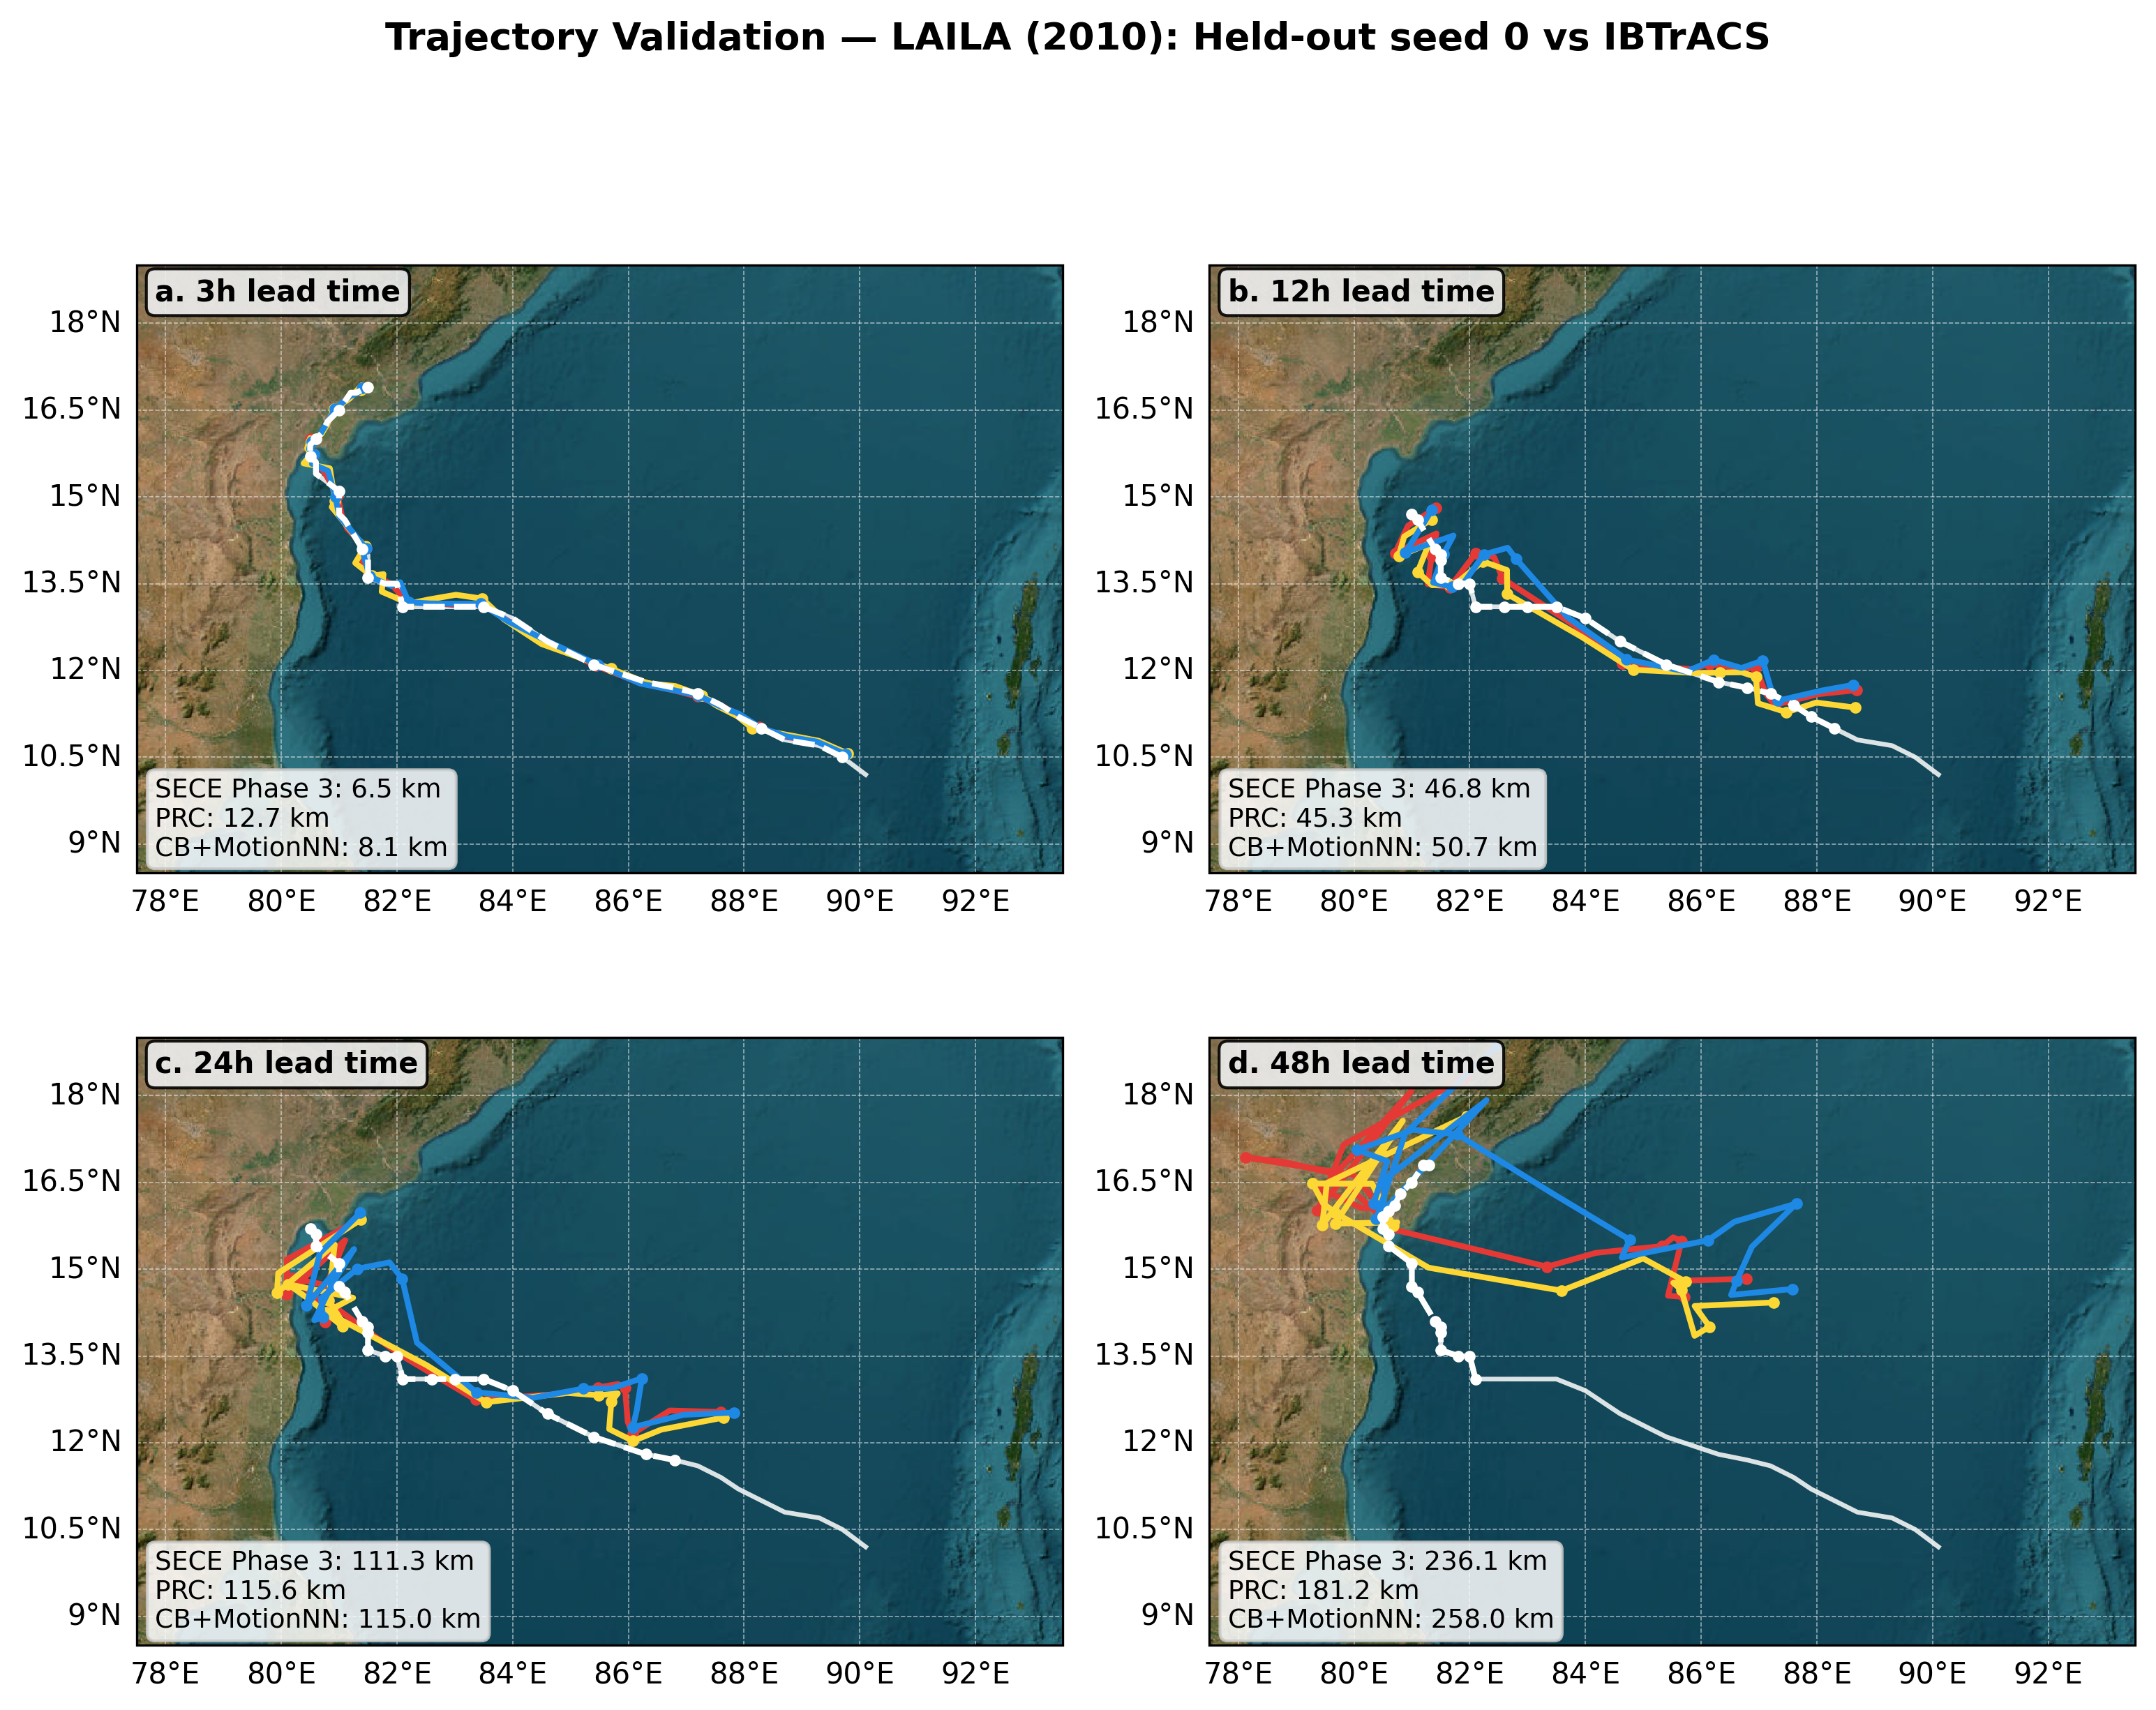
\includegraphics[width=\linewidth]{Figures/case_study_laila_trajectories.png}
\caption{Cyclone Laila (2010) on held-out seed~0. Each marker is a prediction
made from a distinct origin time along the track and offset forward by the
panel's lead time, so panels show direct multi-horizon endpoints rather than a
recursively rolled-out trajectory. Four panels: 3, 12, 24, and 48\,h lead times.}
\label{fig:laila}
\end{figure}

\subsection{Case study}
Fig.~\ref{fig:laila} shows Cyclone Laila (2010), the storm with the largest
single-storm \era{} benefit in the diagnostic above: 25.0\,km at 24\,h and
107.0\,km at 48\,h. At the ensemble level on this storm \sece{} reaches 111.3\,km
at 24\,h against 128.9\,km for the pooled-best competitor, while at 48\,h the
ordering reverses and XGBoost leads locally, 204.9 against 236.1\,km, mirroring
the aggregate leaderboard. A representative storm chosen because its \sece{}
error sits closest to the seed median, an unnamed 1996 system with central-basin
genesis, shows a tighter contest at 24\,h, 107.2 against 110.7\,km. Per-storm
behaviour therefore illustrates the mechanism but does not substitute for pooled
medians.

% =============================================================================
\section{Discussion}
% =============================================================================
The central finding is horizon-dependent. \sece{}'s routed experts deliver a
robust advantage at 3--12\,h, where recurvature, coastal proximity, and steering
are strongly informative; at 24--48\,h, leading tree stacks are statistically
indistinguishable~\cite{grinsztajn2022tree,ganaie2022ensemble,goerss2000tropical,goerss2004tropical}.
\emph{Architectural} and \emph{atmospheric} gains peak at different leads:
subset fusion helps most at short range, whereas Section~V-C shows \era{}
benefit concentrating at 48\,h as persistence weakens~\cite{giffard2020tropical}.
The environ expert bridges the two---it repaired 24\,h ensemble balance in
development (Table~\ref{tab:abl}) rather than dominating every per-storm
diagnostic.

The leakage correction is part of the claim: test-set-guided phase changes did not
replicate on fresh seeds; a frozen design and disjoint held-out tier were
required~\cite{cawley2010}. For the \bob{} rim, at 3--12\,h \sece{} is a defensible default on
reanalysis-collocated tree features without a full NWP suite; at 24--48\,h,
stacking, XGBoost, PRC, and \sece{} overlap within confidence intervals, so
consensus display beats branding one learner dominant. CatBoost-family models
lag at short range but add diversity as ensemble members.

Official NIO track verification (IMD/RSMC; 124/202\,km mean at 24/48\,h in
2009--2013~\cite{mohapatra2013imdtrack}) uses a different protocol than our
IBTrACS hindcast (101/246\,km \sece{} medians); the numbers are not directly
comparable, and we rank ML systems under one frozen protocol rather than claiming
operational consensus-model skill.

Pre-correction architecture sweeps once appeared to win at every horizon on a
single split; that ordering did not replicate on fresh held-out seeds until Phase~3
and the evaluation firewall were frozen~\cite{cawley2010}. Reporting that failure
mode matters for iterative ensemble papers: fusion-path or router choices driven by
test-set rank tables can inflate benchmarks even when no learner reads a test label.

For practitioners, the actionable reading is lead-specific. Routed \sece{} fusion
merits priority at 3--12\,h, where Bonferroni tests show stable separation from
every baseline; at 24--48\,h, display consensus among stacking, XGBoost, PRC, and
\sece{} rather than branding one tree learner dominant. Once \era{} is
pre-collocated at track points, the full eight-system confirm remains feasible on
modest CPU hardware---relevant where full dynamical suites are capacity-limited
along the \bob{} rim~\cite{kumar2024machine,dube2009storm}.

% =============================================================================
\section{Limitations}
% =============================================================================
\textbf{Environmental fields.} The locked model uses \era{} only at the storm
centre (14 point variables). We tested 5$^\circ$/3$^\circ$ spatial-patch
statistics in development; they did not improve 24--48\,h mean error enough to
justify adoption (Table~\ref{tab:abl}, ${\sim}$0.4\,km vs.\ the environ expert,
inside seed noise). Ocean heat content, higher vertical resolution, and forward NWP
as distinct from retrospective reanalysis were not incorporated. Gridded or
attention-based encoders~\cite{giffard2020tropical,qu2025accurate,vaswani2017attention} remain outside this benchmark.

\textbf{Deterministic outputs.} Every system returns a single track point without
forecast spread, which matters most at 24--48\,h where Table~\ref{tab:held} shows
overlapping leading medians and right-skewed errors; proper probabilistic scores~\cite{gneiting2007} are future work.

\textbf{Baseline scope.} The confirm table is an eight-way tree and hybrid
comparison. CNN-GRU and BLSTM were not re-trained on the locked \era{} protocol;
Section~I summarises why exploratory development under the uniform budget did not
justify that cost~\cite{grinsztajn2022tree}. Tuned deep encoders on gridded
\era{} remain future work.

\textbf{Basin and era scope.} Training and confirm use North Indian Ocean storms
with \bob{} exposure; router menus reflect regional steering (monsoon trough,
land proximity). We report no zero-shot or retrained evaluation on the Western
North Pacific, Atlantic, or other basins---cross-basin transfer remains future
work. Genesis 1940--2024 spans pre-satellite and modern records; although a fixed
modern holdout supports the wide window for track error, pre-1979 wind sparsity
limits intensity-adjacent interpretation and residual era confounding cannot be
fully excluded.

\textbf{Attribution.} Section~V-C reports LightGBM \emph{gain} on the environ
expert for held-out seed~0 only. Shear and steering components are collinear by
construction (shear uses the same wind levels as steering), so rank order within
that block is not mechanistic proof; multi-seed SHAP or grouped permutation tests
would be needed for stable within-block attribution.

\textbf{Future work.} Three directions could narrow the 24--48\,h parity band without
relaxing the confirm firewall: physics-constrained displacement models;
probabilistic ensemble tracks scored with proper rules~\cite{gneiting2007}; and
end-to-end attention over storm history plus gridded \era{} rather than point
collocation~\cite{qu2025accurate,giffard2020tropical}. Each should be trained and
ranked under the same storm-wise, multi-seed held-out export used here.

% =============================================================================
\section{Conclusion}
% =============================================================================
We report a leakage-corrected, \era{}-augmented North Indian Ocean benchmark in
which \sece{} Phase~3 wins at 3--12\,h with Bonferroni significance, ties leading
tree stacks at 24--48\,h, and documents rejected spatial patches. Held-out medians
are 4.895, 35.538, 101.186, and 246.331\,km at 3, 12, 24, and 48\,h; \sece{} is
never significantly worse than any evaluated baseline at any horizon, while
CatBoost and CB+MotionNN remain the most consistently outperformed comparators at
short lead. We document controlled \era{} ablation, rejected spatial patches, and
corrected test-set leakage encountered during our own development so follow-on work
can adopt the same storm-wise, multi-seed discipline instead of repeating
single-split leaderboard claims. Natural extensions---probabilistic tracks under
proper scoring rules, gridded \era{} encoders, and cross-basin transfer---should
be evaluated under an equally explicit confirm firewall~\cite{gneiting2007,cawley2010}.

\section*{Acknowledgment}
The authors thank [funding agencies] for support; \era{} data were obtained from
the Copernicus Climate Data Store~\cite{hersbach2023era5}.

\bibliographystyle{IEEEtran}
\renewcommand{\IEEEbibitemsep}{2pt plus 0.6pt}
\begin{thebibliography}{41}

\bibitem{knapp2010ibtracs}
K. R. Knapp, M. C. Kruk, D. H. Levinson, H. J. Diamond, and C. J. Neumann, ``The International Best Track Archive for Climate Stewardship (IBTrACS): Unifying tropical cyclone best track data,'' \textit{Bulletin of the American Meteorological Society}, vol. 91, no. 3, pp. 363--376, Mar. 2010.

\bibitem{gahtan2024ibtracs}
J. Gahtan, K. R. Knapp, C. J. Schreck, H. J. Diamond, and J. P. Kossin, ``International Best Track Archive for Climate Stewardship (IBTrACS) Project, Version 4r01,'' NOAA National Centers for Environmental Information, 2024. [Online]. Available: https://doi.org/10.25921/82ty-9e16

\bibitem{worldbank2007sidr}
World Bank, ``Cyclone Sidr in Bangladesh: Damage, Loss, and Needs Assessment for Disaster Recovery and Reconstruction,'' Washington, DC, USA, Tech. Rep., 2007.

\bibitem{paul2013post}
S. Paul, ``Post-cyclone livelihood status and strategies in coastal Bangladesh,'' \textit{Rajshahi University Journal of Life \& Earth and Agricultural Sciences}, vol. 41, pp. 1--20, 2013.

\bibitem{lian2020novel}
J. Lian, P. Dong, Y. Zhang, J. Pan, and K. Liu, ``A novel data-driven tropical cyclone track prediction model based on CNN and GRU with multi-dimensional feature selection,'' \textit{IEEE Access}, vol. 8, pp. 97114--97128, 2020. doi: 10.1109/ACCESS.2020.2992083.

\bibitem{alemany2019predicting}
S. Alemany, J. Beltran, A. Perez, and S. Ganzfried, ``Predicting hurricane trajectories using a recurrent neural network,'' in \textit{Proc. AAAI Conf. Artificial Intelligence}, vol. 33, Honolulu, Hawaii, USA, 2019, pp. 468--475.

\bibitem{giffard2020tropical}
S. Giffard-Roisin, M. Yang, G. Charpiat, C. K. Bonfanti, B. K\'{e}gl, and C. Monteleoni, ``Tropical cyclone track forecasting using fused deep learning from aligned reanalysis data,'' \textit{Frontiers in Big Data}, vol. 3, p. 1, Jan. 2020.

\bibitem{kar2021tropical}
C. Kar and S. Banerjee, ``Tropical cyclone intensity prediction using best track data over North Indian Ocean by machine learning classifiers,'' in \textit{2021 IEEE International India Geoscience and Remote Sensing Symposium (InGARSS)}, pp. 297--300, Dec. 2021.

\bibitem{goerss2004tropical}
J. S. Goerss, ``Tropical Cyclone Track Forecasts Using an Ensemble of Dynamical Models,'' \textit{Weather and Forecasting}, vol. 19, no. 2, pp. 255--263, Apr. 2004.

\bibitem{ganaie2022ensemble}
M. A. Ganaie, M. Hu, A. K. Malik, M. Tanveer, and P. N. Suganthan, ``Ensemble deep learning: A review,'' \textit{Engineering Applications of Artificial Intelligence}, vol. 115, p. 105151, Nov. 2022.

\bibitem{grinsztajn2022tree}
L. Grinsztajn, E. Oyallon, and G. Varoquaux, ``Why do tree-based models still outperform deep learning on tabular data?,'' in \textit{Proc. 36th Int. Conf. Neural Inf. Process. Syst. (NeurIPS)}, 2022, pp. 507--520.

\bibitem{neumann1972alternative}
C. J. Neumann, ``An alternate to the HURRAN (Hurricane Analog) Tropical Cyclone Forecast System,'' \textit{NOAA Technical Memorandum}, NWS SR-62, 1972.

\bibitem{dube2009storm}
S. K. Dube, I. Jain, A. D. Rao, and T. S. Murty, ``Storm surge modelling for the Bay of Bengal and Arabian Sea,'' \textit{Natural Hazards}, vol. 51, pp. 3--27, Oct. 2009, doi: 10.1007/s11069-009-9397-9.

\bibitem{mohapatra2013imdtrack}
M. Mohapatra, D. P. Nayak, R. Sharma, and B. K. Bandyopadhyay, ``Evaluation of official tropical cyclone track forecast over north Indian Ocean issued by India Meteorological Department,'' \textit{J. Earth Syst. Sci.}, vol. 122, no. 3, pp. 589--601, 2013, doi: 10.1007/s12040-013-0291-1.

\bibitem{aberson1998five}
S. D. Aberson, ``Five-day tropical cyclone track forecasts in the North Atlantic basin,'' \textit{Weather and Forecasting}, vol. 13, no. 4, pp. 1005--1015, Dec. 1998.

\bibitem{goerss2000tropical}
J. S. Goerss, ``Tropical cyclone track forecasts using an ensemble of dynamical models,'' \textit{Monthly Weather Review}, vol. 128, no. 4, pp. 1187--1193, Apr. 2000.

\bibitem{hossain2021track}
M. S. Hossain, M. A. Samad, M. R. Sultana, M. Mallik, and M. J. Uddin, ``Track and Landfall Characteristics of Very Severe Cyclonic Storm Fani over the Bay of Bengal using WRF Model,'' \textit{Dhaka University Journal of Science}, vol. 69, no. 2, pp. 101--108, Dec. 2021.

\bibitem{rahman2025tropical}
S. Rahman \textit{et al.}, ``Tropical cyclone track prediction harnessing deep learning algorithms: A comparative study on the Northern Indian Ocean,'' \textit{Results in Engineering}, vol. 26, Art.\ no.\ 105009, 2025.

\bibitem{kumar2024machine}
S. Kumar, A. K. Singh, and R. K. Jaiswal, ``Machine learning-based tropical cyclone track and intensity prediction: A comprehensive review,'' \textit{Natural Hazards Review}, vol. 25, no. 2, p. 03124001, 2024.

\bibitem{qu2025accurate}
H. Qu, H. Xu, L. Dong, C. Xiang, and G. Nie, ``Accurate typhoon intensity forecasts using a non-iterative spatiotemporal transformer model,'' arXiv preprint arXiv:2509.21349, Sep. 2025.

\bibitem{chen2016xgboost}
T. Chen and C. Guestrin, ``XGBoost: A scalable tree boosting system,'' in \textit{Proc. 22nd ACM SIGKDD Int. Conf. Knowledge Discovery and Data Mining}, San Francisco, CA, USA, 2016, pp. 785--794.

\bibitem{ke2017lightgbm}
G. Ke, Q. Meng, T. Finley, T. Wang, W. Chen, W. Ma, Q. Ye, and T. Y. Liu, ``LightGBM: A Highly Efficient Gradient Boosting Decision Tree,'' in \textit{Proc. 31st Int. Conf. Neural Inf. Process. Syst. (NIPS)}, 2017, pp. 3149--3157.

\bibitem{prokhorenkova2018catboost}
L. Prokhorenkova, G. Gusev, A. Vorobev, A. V. Dorogush, and A. Gulin, ``CatBoost: unbiased boosting with categorical features,'' in \textit{Proc. 32nd Int. Conf. Neural Inf. Process. Syst. (NeurIPS)}, 2018, pp. 6638--6648.

\bibitem{hersbach2023era5}
H. Hersbach et al., ``ERA5 hourly data on single levels from 1940 to present,'' Copernicus Climate Change Service (C3S) Climate Data Store (CDS), 2023. [Online]. Available: https://doi.org/10.24381/cds.adbb2d47

\bibitem{krishnamurti2010ann}
T. N. Krishnamurti, A. K. Mishra, A. Simon, A. Semazzi, and H. S. Bhardwaj, ``Predicting cyclone tracks in the north Indian Ocean: An artificial neural network approach,'' \textit{Geophys. Res. Lett.}, vol. 37, no. 20, L19801, 2010, doi: 10.1029/2010GL044718.

\bibitem{breiman2001rf}
L. Breiman, ``Random forests,'' \textit{Machine Learning}, vol. 45, no. 1, pp. 5--32, Oct. 2001, doi: 10.1023/A:1010933404324.

\bibitem{maaten2008tsne}
L. van der Maaten and G. Hinton, ``Visualizing data using t-SNE,'' \textit{Journal of Machine Learning Research}, vol. 9, pp. 2579--2605, 2008.

\bibitem{vaswani2017attention}
A. Vaswani, N. Shazeer, N. Parmar, J. Uszkoreit, L. Jones, A. N. Gomez, \L. Kaiser, and I. Polosukhin, ``Attention is all you need,'' in \textit{Advances in Neural Information Processing Systems}, vol. 30, Long Beach, CA, USA, 2017.

\bibitem{cawley2010}
N. J. Cawley and G. C. L. Talbot, ``On Over-fitting in Model Selection and Subsequent Selection Bias in Performance Evaluation,'' \textit{Journal of Machine Learning Research}, vol. 11, pp. 2079--2107, 2010.

\bibitem{efron1979}
B. Efron, ``Bootstrap Methods: Another Look at the Jackknife,'' \textit{The Annals of Statistics}, vol. 7, no. 1, pp. 1--26, 1979.

\bibitem{wilcoxon1945}
F. Wilcoxon, ``Individual Comparisons by Ranking Methods,'' \textit{Biometrics Bulletin}, vol. 1, no. 6, pp. 80--83, Dec. 1945.

\bibitem{bonferroni1936}
C. E. Bonferroni, ``Teoria statistica delle classi e calcolo delle probabilit\`a,'' \textit{Pubblicazioni del R Istituto Superiore di Scienze Economiche e Commerciali di Firenze}, vol. 8, pp. 3--62, 1936.

\bibitem{sinnott1984}
R. W. Sinnott, ``Virtues of the Haversine,'' \textit{Sky and Telescope}, vol. 68, no. 2, p. 159, 1984.

\bibitem{gneiting2007}
T. Gneiting and A. E. Raftery, ``Strictly Proper Scoring Rules, Prediction, and Estimation,'' \textit{Journal of the American Statistical Association}, vol. 102, no. 477, pp. 359--378, 2007.

\end{thebibliography}

\end{document}
